\documentclass[a4paper]{article}
\usepackage{fullpage}
\usepackage{amsfonts}
\usepackage{amsmath}
\usepackage{graphicx}
\usepackage{amsthm}


\newtheorem{thm}{Theorem}

\graphicspath{ {/home/aurelien/} }

\title{Data adaptive selection of the truncation level}

\begin{document}

\maketitle

\section{Problem setting}

For a single time point intervention, assume $W$ is univariate and continuous.

Denote $\Psi_0(\delta) = E_{P_0}\left[\frac{g_0(d(W)|W)}{g_{0, \delta}(d(W)|W)}Q_{Y,0}(d(W), W)\right]$.
 
Under the proper causal assumptions, $\Psi_0(0) = EY^d$.

Let $\delta_n = \text{argmin}_\delta MSE_n(\delta) \equiv \text{argmin}_\delta E_{P_0} \left(\Psi_{n, g_n}(\delta)(\delta) - EY^d\right)^2$.


We'd like to find a method that would data-adaptively select a truncation level $\hat{\delta}_n$ such that $MSE_n(\hat{\delta}_n) \sim MSE_n(\delta_n)$.

Minimizing $MSE_n(\delta)$ (w.r.t. $\delta$) from the data is tough: we would have to estimate the $MSE'_n(\delta)$ which involves $(b_0^2)'(\delta) = 2  b_0(\delta) b_0'(\delta)$. Since bias is necessarily as hard to estimate as $EY^d$ itself, estimating $MSE'_n(\delta)$ should be hard too.

We have to find a surrogate risk that is easier to estimate from the data. Let $R_n(\delta) = b_0(\delta) + \frac{1}{\sqrt{n}} \sigma_0(\delta)$. This risk might be easier to estimate, since $b_0'(\delta)$ should be close to the finite difference $\frac{\Psi_0(\delta + \Delta) - \Psi_0(\delta)}{\Delta}$. Since for $\delta$ large enough $\Psi_0(\delta)$ and $\Psi_0(\delta + \Delta)$ are "easy" to estimate, there's hope we can estimate the finite difference.

\textbf{We've convinced ourselves that  $\delta_n^* \equiv \text{argmin}_\delta \sim \delta_n$ (we sketched a proof of this over email)}.

\medskip

\section{A method to find $\hat{\delta}_n \sim \delta_n$}

\subsection{Estimating $b'_0(\delta)$}

Define the "true finite difference" $\Delta b_0(\delta) = \frac{b_0(\delta + \Delta) - b_0(\delta)}{\Delta}$

Denote the estimated finite difference $\widehat{\Delta b}_n(\delta) = \frac{\hat{b}_n(\delta + \Delta) - \hat{b}_n(\delta)}{\Delta} = \frac{\hat{\Psi}_n(\delta + \Delta) - \hat{\Psi}_n(\delta)}{\Delta}$.

\medskip

Assume there exist $1 > \beta \geq 0$ and $1/2 > \gamma \geq 0$ such that $b_0(\delta) \sim \delta^{1 - \beta}$, $b_0'(\delta) \sim \delta^{-\beta}$, $\beta_0''(\delta) \sim \delta^{-\beta - 1}$, $\sigma_0(\delta) \sim \delta^{-\gamma}$, and $\sigma'_0(\delta) \sim \delta^{-\gamma - 1}$. Assume also that $\beta < \gamma + 1$.

Under these assumptions, $R'(\delta_n^*) = 0$ implies that $\delta^{-\beta}  + \frac{1}{\sqrt{n}} \delta^{-\gamma} = 0$, i.e. $\delta_n^* \sim n^{-\frac{1}{2(\gamma + 1 - \beta)}}$.

\smallskip

The typical error we make in estimating $b_n'(\delta)$, which I'll denote $\sigma_{b'_0(\delta), n}$, is the statistical error plus the approximation error. The approximation error is $\Delta b''(\delta) + o(\Delta)$. The standard deviation of $\widehat{\Delta b_n}(\delta)$ can be upper bounded by $n^{-1/2} \Delta^{-1} \sigma_0(\delta)$. Therefore
$$\sigma_{b'_0(\delta), n} = \Delta b''(\delta) + n^{-1/2} \Delta^{-1} \sigma_0(\delta) \sim \Delta \delta^{-\beta - 1} + \Delta^{-1} n^{-1/2} \delta^{-\gamma}.$$


For a given $\delta$ and a given $n$, let's optimize it wrt $\Delta$. Setting $ \frac{d}{d \Delta} \sigma_{b'_0(\delta), n, \Delta} = 0$ yields $\Delta(n, \delta) \sim n^{-1/4} \delta^\frac{\beta + 1 - \gamma}{2}$. For this choice of $\Delta$, $\sigma_{b'_0   (\delta^*_n), n, \Delta} \sim n^{-1/4} \delta^{-\frac{\gamma + 1 + \beta}{2}}$.


We need the $\sigma_{b'_0(\delta), n} << b'_0(\delta)$ to be able to estimate $b'0_{\delta}$ from the finite difference $\widehat{b_n}(\delta)$. For the optimal choice $\Delta(n, \delta)$, and \textbf{for $\delta$ small, $\sigma_{b'_0(\delta), n} << b'_0(\delta)$ is equivalent to $\delta >> \delta_n^*$}.

\textbf{Thus, if we are to estimate anything related to $b'_0(\delta)$, we need to it at a $\tilde{\delta}_n$ such that $\tilde{{\delta}_n} = o(\delta_n^*)$}

\subsection{Estimating the rate in $\delta$ of $\sigma_0(\delta)$}


Estimating the rate in $\delta$ of $\sigma_0(\delta)$ seems to be feasible. 
For various samples sizes and for a few target parameters, I plotted the $\log \sigma_n(\delta)$ against $log(\delta)$, where $\sigma_n(\delta)$ is the empirical variance of the influence curve.

In my simulations I worked with a family of data-generating distributions defined by:

\begin{align*}
W &\sim Exp\left(\frac{1}{\lambda} \right)\\
A &\sim Bernouilli(expit(\alpha_0 W)) \\
Y &\sim Bernouilli(expit(\beta_0 + \beta_1 A+ \beta_2 W))
\end{align*}

\textbf{True rates for these data generating distributions:}

If $\beta_2 > 0$, $b_0(\delta) \sim \delta^{-1 + \frac{\lambda^{-1} + \alpha_0 + \beta_2}{\alpha_0}}$ and thus $\beta = 2 - \frac{\lambda^{-1} + \alpha_0 + \beta_2}{\alpha_0}$. Also, $\sigma_0^2(\delta) = \delta^{-2 + \frac{\lambda^{-1} + \alpha_0 + \beta_2}{\alpha_0}}$ and thus $\gamma = 1 - \frac{\lambda^{-1} + \alpha_0 + \beta_2}{\alpha_0}$.
The optimal rate is then $\frac{\alpha_0}{\alpha_0 + \lambda^{-1} + \beta_2}$.

If $\beta_2 < 0$, $b_0(\delta) \sim \delta^{-1 + \frac{\lambda^{-1} + \alpha_0}{\alpha_0}}$ and thus $\beta = 2 - \frac{\lambda^{-1} + \alpha_0}{\alpha_0}$. Also, $\sigma_0^2(\delta) = \delta^{-2 + \frac{\lambda^{-1} + \alpha_0 + |\beta_2|}{\alpha_0}}$ and thus $\gamma = 1 - \frac{\lambda^{-1} + \alpha_0 + |\beta_2|}{\alpha_0}$.
The optimal rate is then $\frac{\alpha_0}{\alpha_0 + \lambda^{-1} - |\beta_2|}$.

\bigskip

Here is what I got for $(\lambda, \alpha_0, \beta_0, \beta_1, \beta_2) = (2, 2, -3, 1.5, 1)$ and $(\lambda, \alpha_0, \beta_0, \beta_1, \beta_2) = (2, 4, -3, 1.5, 0.5)$. These specifications of the data-generating distribution make $EY_1$ weakly identifiable.

\begin{figure}[!htbp]
   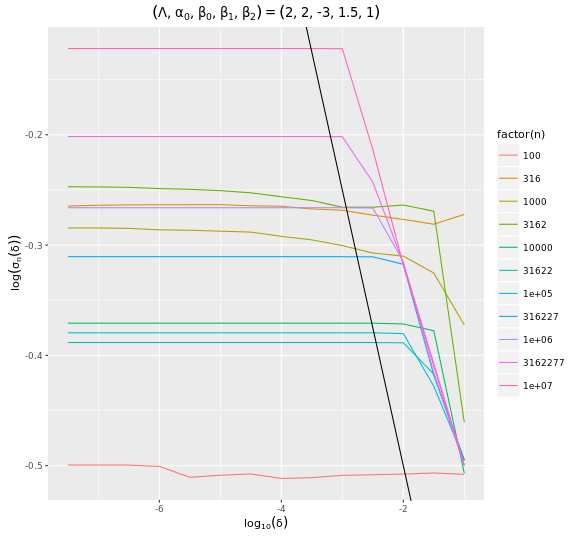
\includegraphics[scale = 0.4]{sigm_n(delta)-hard-tp.png}
\end{figure}

\begin{figure}[!htbp]
   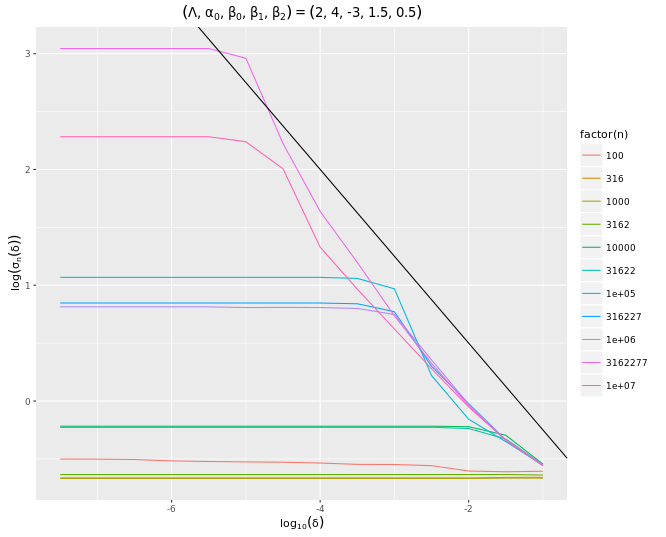
\includegraphics[scale = 0.35]{sigm_n(delta)-easy-tp.png}
\end{figure}

The black line has the true rate $\gamma$ as slope. Seems like for $n > 1e3$ we should be able to estimate $\gamma$ decently well from our data, just by fitting a line to $\sigma_n(\delta)$ in a region where $\delta$ is neither too big (so that the behavior of $\sigma_0(\delta)$ is asymptotic) and neither too small (so that we have asymptotic linearity of our TMLE).

\subsection{Estimating the rate of $\delta_n$}

Assume that we can estimate the rate $-\gamma$ of $\sigma_0(\delta)$ (see above section regarding feasibility of this).

For $\eta > 1$, let $\delta_{n, \eta} = n^{-\frac{1}{2 \eta (\gamma + 1 - \beta)}}$.

Assume that $\Psi_n(\delta_{\eta, n}) \sim \Psi_0(\delta_n{\eta, n}) + P_n D_\delta(P_0)(O)$. This should be fine for $\delta_n{\eta, n}$ slow enough (i.e. for $\eta$ large enough).

Let $g_{\eta, n}(\delta) = \sqrt{n} \left( \widehat{\Delta b_n}(\delta) \delta^{\gamma + 1} \right)^\eta$.

We have that $g_{\eta, n}(\delta_{n, \eta - \epsilon}) \sim C^\eta n^{-\frac{\epsilon}{2(\eta - \epsilon)}} \rightarrow 0$, $g_{\eta, n}(\delta_{n, \eta + \epsilon}) \sim C^\eta n^{\frac{\epsilon}{2(\eta + \epsilon)}} \rightarrow \infty$, and $g_{\eta, n}(\delta_{n, \eta}) \rightarrow C^\eta$, for a certain constant $C$.

This suggests two different methods to estimate the optimal rate $\frac{-1}{2(\gamma + 1 - \beta)}$.

\paragraph{First method.} Let $\eta > 1$. Solve $g_{\eta, n}(\delta) = 1$. The solution is $\sim n^{-\frac{1}{2(\gamma + 1 - \beta)}}$. Simulations show that the existence of a solution can require an extremely high $n$, since the constant $\eta |\log C|$ can be large.

\paragraph{Second method.} Since the constant $C$ is problematic, another option is to check for different rates $r_1, ..., r_q$ whether $g_{\eta, n}(n^{-r_i})$ is increasing, decreasing or stationary as $n$ increases.

To be able to do this, we need to compare $g_{n, n^{-r_i}}$ for different values of $n$. This suggest the following method. Let $\mathcal{O}_n$ our sample. Let $\mathcal{O}_{\tilde{n}}^1$,..., $\mathcal{O}_{\tilde{n}}^m$ $m$ subsamples of $\mathcal{O}$ of size $\tilde{n}$ (in my simulations I worked with $\tilde{n} = n / 3$ and $\tilde{n} = n / 10$). Compute the median of $\{g_{\eta, n, \mathcal{O}_n}(n^{-r_i}) - g_{\eta, \tilde{n}, \mathcal{O}_{\tilde{n}}^k}(\tilde{n}^{-r_i}) : k \in \{1,...,m\} \}$. If for the rates $r_i$ and $r_{i + 1}$ this median is respectively positive and negative, then we estimate the optimal rate by a value between $r_i$ and $r_{i+1}$.

We can refine the interval $[r_i, r_{i+1}]$ such that we find a rate $r$ for which we have stationarity of $g_{\eta, n}(n^{-r}$ from our subsamples to our full sample.


I did a bunch of simulations for the family of data-generating distribution specified above. 

Here are some encouraging plots (figures 1 and 2).

\begin{figure}[!htbp]
	\caption{$\log g_{n, \eta}(n^{-r / \eta})$ (y axis) for $r \in \{0.95 r^{optimal}, r^{optimal}, 1.05 r^{optimal} \}$, for various values of $\eta$. We observe that the stationary curves are the ones that correspond to $r^{optimal}$. x axis is $log(\delta)$}
   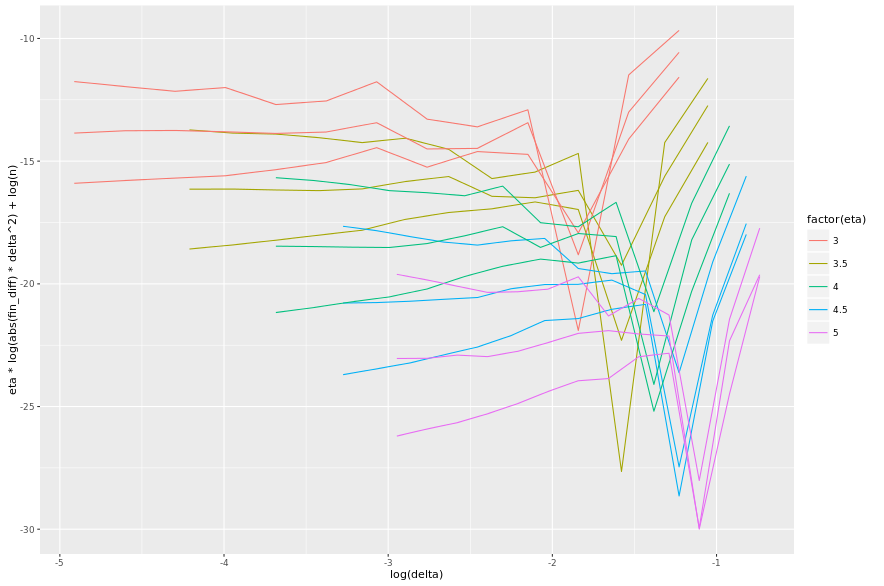
\includegraphics[scale = 0.4]{LHS-bracketing_of_delta_n^star-easy-tp.png}
\end{figure}

\begin{figure}[!htbp]
	\caption{$\log g_{n, \eta}(n^{-r / \eta})$ (y-axis) from $n = 10^7$ to $n=10^8$, for various candidate rates. x-axis: $\log \delta$. The optimal rates lies between two consecutive candidates rates for which we observe the slopes to change sign. That's good.}
   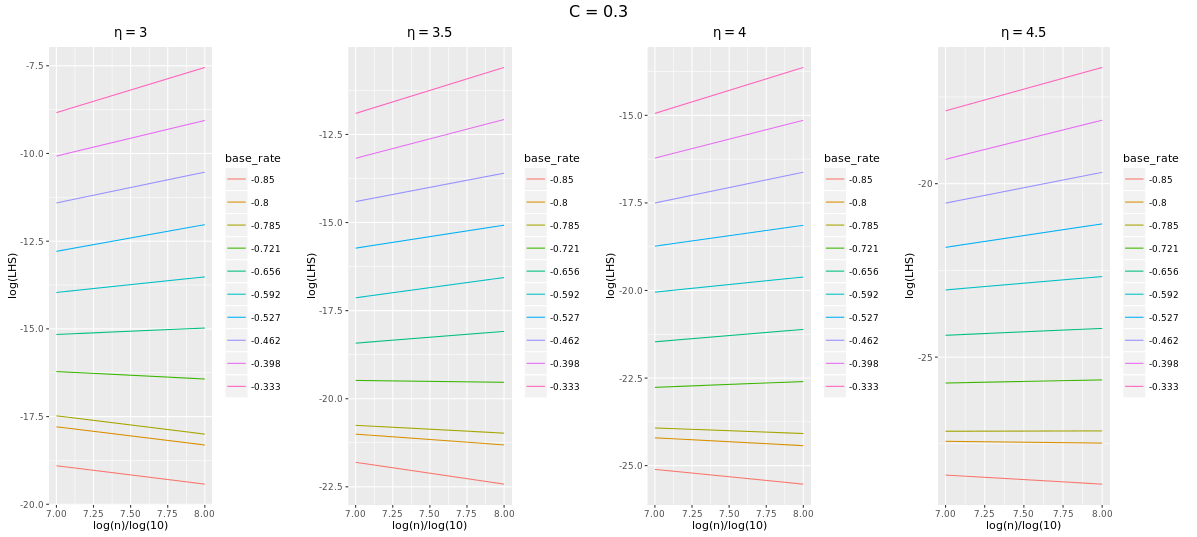
\includegraphics[scale = 0.4]{rates_comb-easy-tp-1e7to1e8.png}
\end{figure}

\bigskip

\subsection{Remark on selection of the step of the finite difference} 

We need to know $\beta$ and $\gamma$ to know the optimal $\Delta(n, \delta)$.
We can probably access $\gamma$ (the rate of $\sigma_0(\delta)$) directly from the data, but it seems much harder to do so for $\beta$.

We probably don't need $\Delta$ to be optimal to have $\sigma_{b_0'(\delta^*_n),n} = o(b_0'(\delta^*_n))$.

A suggestion is to act as if $\beta$ was $\gamma + 1- \tilde{\epsilon}$ for a small $\epsilon \in (0, \gamma + 1 - \beta)$ (but closer to zero than to $\gamma + 1 - \beta)$. We assume that $\gamma$ is known. Let's see where this leads:

The "optimal" $\Delta$ we would pick is then given by

$$\Delta^2 = \frac{n^{-1/2} \delta^{-\gamma}}{\delta^{-(\gamma + 1 - \tilde{\epsilon}) - 1}} = n^{-1/2} \delta^{2 - \tilde{\epsilon}}$$

i.e. $\Delta = n^{-1/4} \delta^{1 - \tilde{\epsilon}/2}$.

Let $(\delta_n^+)_{n \geq 1}$ be such that $\delta_n^+ = o(\delta_n)$. Now let's check if we have $\sigma_{b_0'(\delta^+_n),n} = o(b_0'(\delta^+_n))$.

We have

\begin{align*}
\sigma_{b_0'(\delta^+_n),n} &= \Delta {\delta^+_n}^{-\beta - 1} + n^{-1/2} {\delta^+_n}^{-\gamma} \Delta^{-1}\\
&=n^{-1/4} {\delta^+_n}^{-\beta - \tilde{\epsilon}/2} + n^{-1/4} {\delta^+_n}^{-\gamma - \tilde{\epsilon} / 2 - 1} \\
&= n^{-1/4} \left({\delta^+_n}^{-(\beta + \tilde{\epsilon} / 2)} + {\delta^+_n}^{-(\gamma + 1 - \tilde{\epsilon} / 2)} \right)
\end{align*}

Since we pick $\tilde{\epsilon}$ relatively small we have $\gamma + 1 - \tilde{\epsilon} / 2 >  \beta + \tilde{\epsilon} / 2$.

Thus $\sigma_{b_0'(\delta^+_n),n} \sim n^{-1/4} {\delta^+_n}^{-(\beta + \tilde{\epsilon} / 2)} \sim \left(\frac{\delta_n}{\delta_n^+}\right)^{\beta + \tilde{\epsilon}/2} n^\frac{2 \beta - ((\gamma + 1 - \beta) - \tilde{\epsilon})}{4(\gamma + 1 - \beta)}$.

We have $b'_0(\delta^+_n) \sim  \left(\frac{\delta_n}{\delta_n^+}\right)^{\beta} n^\frac{\beta}{2(\gamma + 1 - \beta)}$.

Since $\tilde{\epsilon} < \gamma + 1 - \beta$ we have $\sigma_{b'_0(\delta^+_n)} = o(b'_0(\delta^+_n))$.


\medskip

That's hopeful since picking a small $\tilde{\epsilon}$ is probably practically feasible.

\medskip

\section{Theoeretical result}

Given the above, I guess we can prove the following theorem:

\begin{thm}
Assume there exist $1 > \beta \geq 0$ and $1/2 > \gamma \geq 0$ such that $b_0(\delta) \sim \delta^{1 - \beta}$, $b_0'(\delta) \sim \delta^{-\beta}$, $\beta_0''(\delta) \sim \delta^{-\beta - 1}$, $\sigma_0(\delta) \sim \delta^{-\gamma}$, 
and $\sigma'_0(\delta) \sim \delta^{-\gamma - 1}$. 

Assume also that $\beta < \gamma + 1$.


Denote $\delta_n$ the solution to $MSE_n(\delta) = 0$.


Assume that there exist $\delta_n^+ \rightarrow 0$, such that for any $\tilde{\delta}_n$ that goes to zero slower than $\delta_n^+$, 

\begin{align*}
\hat{\Psi}_n(\tilde{\delta}_n) &\sim \Psi_0(\tilde{\delta}_n) + P_n D^*_{\Psi_0(\tilde{\delta}_n)}.
\end{align*}

Let $\tilde{\epsilon} \in (0, \gamma + 1 - \beta)$, and $\Delta(\delta, n) = n^{-1/4} \delta^{1 - \tilde{\epsilon} / 2}$. Let $\eta > 1$ large enough so that $n^{-\frac{1}{2 \eta (\gamma + 1 - \beta)}}$ goes to zero slower than $\delta_n^+$.

Denote $r_n$ the rate we find using the "second method" above. Then $n^{-r_n} \sim C \delta_n^{1 / \eta}$ for a certain constant $C$, and $MSE_n(n^{-r_n}) \sim C' MSE_n(\delta_n)$ for a certain constant $C'$.

\end{thm}

\section{Discussion}

I need to make this method work well for small sample sizes. Checking asymptotic linearity is key to this.

Shapiro-Wilks test for normality of $Psi_n^(\delta)$ for which I bootstrap the targeting step does not seem to be stringent enough.

For low sample sizes, it's kind of possible to check that things aren't behaving as expected from the asymptotics: the plots of the type of figure 1 and 2 then look messy.

\end{document}